

\setcounter{section}{3}
\section{Hardware Design}
\bigskip
\subsection{System Operation Modes}
\medskip
The Akrievia Beacon system will have two modes of operations, the idle mode, and the emergency mode. Idle mode occurs during every day operation that is not under an emergency. An emergency is defined as a situation that poses an immediate risk to health, life, property, or environment. Most emergencies require urgent intervention to prevent a worsening of the situation. In emergency situations the system will be triggered on to operate under the emergency mode following a system state diagram as shown in figure \ref{sys_state}.

\bigskip
When system is under idle mode, the beacon system does not attempt to transmit location information from ID Tags to the DPU, as the ID Tags will be under deep sleep mode. In idle mode the system is available for configuration such as adding/deleting ID Tags and beacons. In the Event of an emergency, a trigger such as one that could be associated with a fire alarm will trigger the system state into the emergency mode.

\bigskip
When system is under emergency mode, the beacons will attempt to establish a data pipeline using the UWB modules. And the ID Tags are triggered on by personnel carrying the device that are in need of rescue or assistance. Under emergency mode the DPU triggers the Beacons to start sending and receiving packets to determine ToF data from the ID Tags. The ID tags will receive request packet from beacon and transmit location data back to the beacon. Once the emergency situation is resolved the system can be switched back into idle mode.

\medskip
\begin{figure}[H]
\centering
    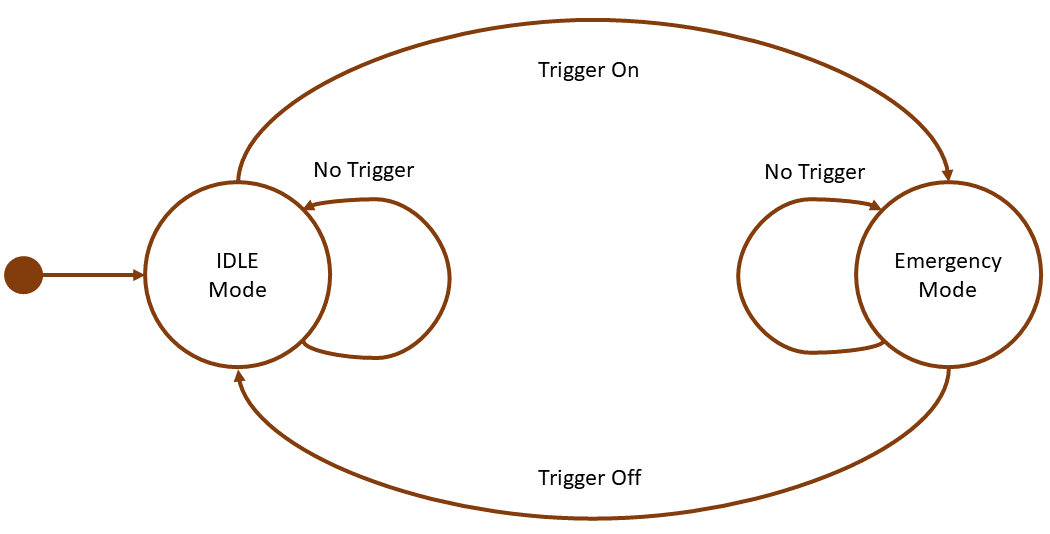
\includegraphics[scale=0.6]{./images/state_d.png}
    \caption{Akriveia Beacon System State Diagram}
    \label{sys_state}
\end{figure}
\medskip



\pagebreak
\subsection{Communication Protocol}
\subsubsection{Beacon to ID Tag Communication}
\medskip
Communication between a beacon and an ID tag is facilitated on the Physical (PHY) layer. The Physical layer is responsible for converting data into bits for transmission and converting received bits back into data.The logical connection formed between the two entities are the radio channels that are present in air. In the proof of concept phase, 2MHz wide BLE advertising channels 37, 38 and 39 with center frequencies at 2402MHz, 2426MHz and 2480MHz respectively can be used \ref{R4-2-3}. In the engineering prototype and final phase, 500MHz wide UWB channels 1, 2, 3 and 5 with center frequencies at 3494MHz, 3993MHz, 4492MHz and 6489MHz respectively can be used \ref{R4-2-2}. The radio channels will be used at full duplex to allow simultaneous transmission in both directions. Digital data such as RSSI measurements, ToF measurements and MAC address are encoded into analog signals by means of modulation to represent the data with continuously varying electromagnetic waves. Modulation in both BLE and UWB form pulses of analog signals prior to transmission \ref{R4-2-3}. The process of sending and receiving these analog signals are handled by the integrated chip antenna of the ESP32 and DWM1000 modules. Upon reception of the analog signals, the receiver's demodulator and decoder will reverse the work of the sender to retrieve the digital data. 
\medskip
\subsubsection{Beacon to DPU Communication}
\medskip
For the proof of concept and prototype, data-pipeline is a simple implementation with USB serial interface. The Beacon and DPU  will listen and send data with the data processing unit over the serial read and write interface. In the Final design the Beacons will use the WiFi module on the ESP32 to join a privately hosted access point created by a hostapd on the data processing unit (Raspberry Pi). Once each beacon is connected to the access point they will be assigned an IP by the Dynamic Host Configuration Protocol (DHCP) server. A one-to-many network will be created as shown in figure \ref{udp}. Using User Datagram Protocol (UDP) communication over the networking layer, the DPU can bind on the gateway IP and a specific port to listen for forwarded beacon data. To initiate control with the beacons, the DPU will bind to each beacon IP at a specified port and send commands using UDP.

\medskip
\begin{figure}[H]
\centering
    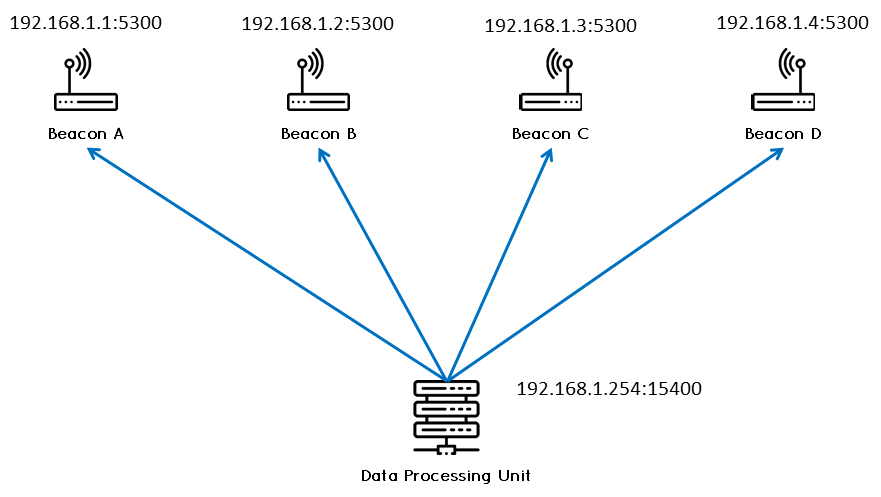
\includegraphics[scale=0.55]{./images/UDP.png}
    \caption{UDP Communication Network}
    \label{udp}
\end{figure}
\medskip



\pagebreak
\subsection{Beacon Design}
The Beacon units, which will relay location data from the ID Tags to the Data Processing Unit (DPU), consist of an ESP32 module, a DWM1000 UWB transceiver, a 9V lithium ion battery, and a power cable. These components will be contained in an encasing made from PLA plastic. This unit will have LEDs indicating the power state, and whether the Beacon is transmitting or receiving, and a reset button. The DPU will send a command to the beacon and the ESP32 will evaluate the command and execute accordingly as shown in figure \ref{bcn_flow}.

\medskip
\begin{figure}[H]
\centering
    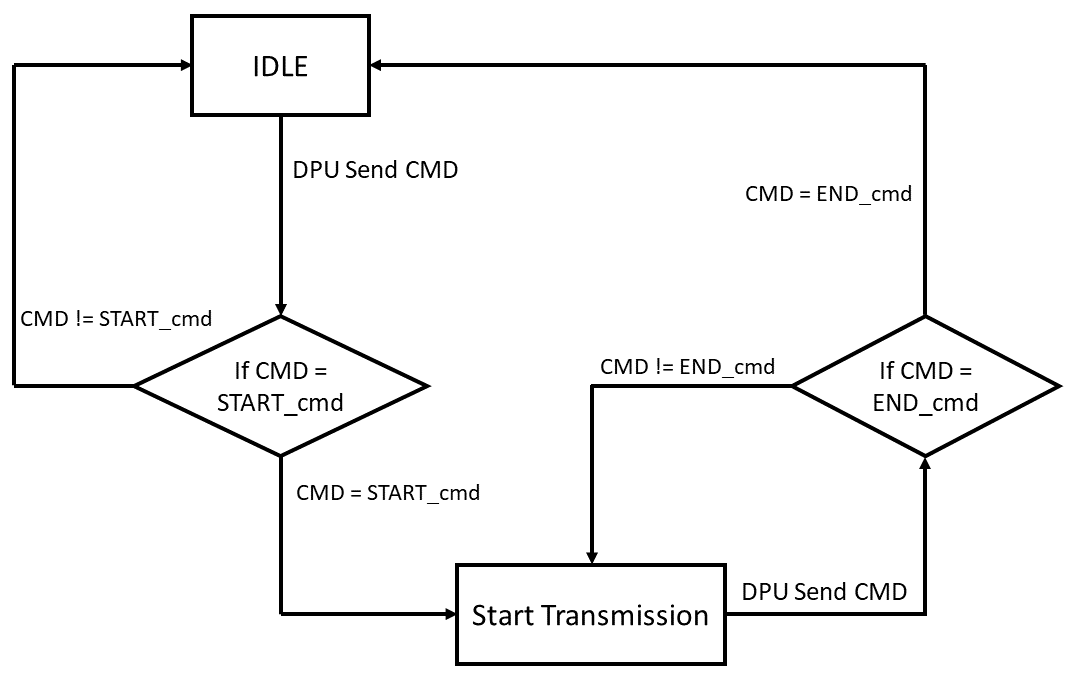
\includegraphics[scale=0.40]{./images/beacon_flow.png}
    \caption{Beacon System Flow Diagram}
    \label{bcn_flow}
\end{figure}
\medskip

A 3D appearance mock-ups of the ID Tag was done in Solidworks and can be seen in the Computer Aided Design (CAD) representation, figure \ref{Bcn_CAD}. 

\medskip
\begin{figure}[H]
\centering
    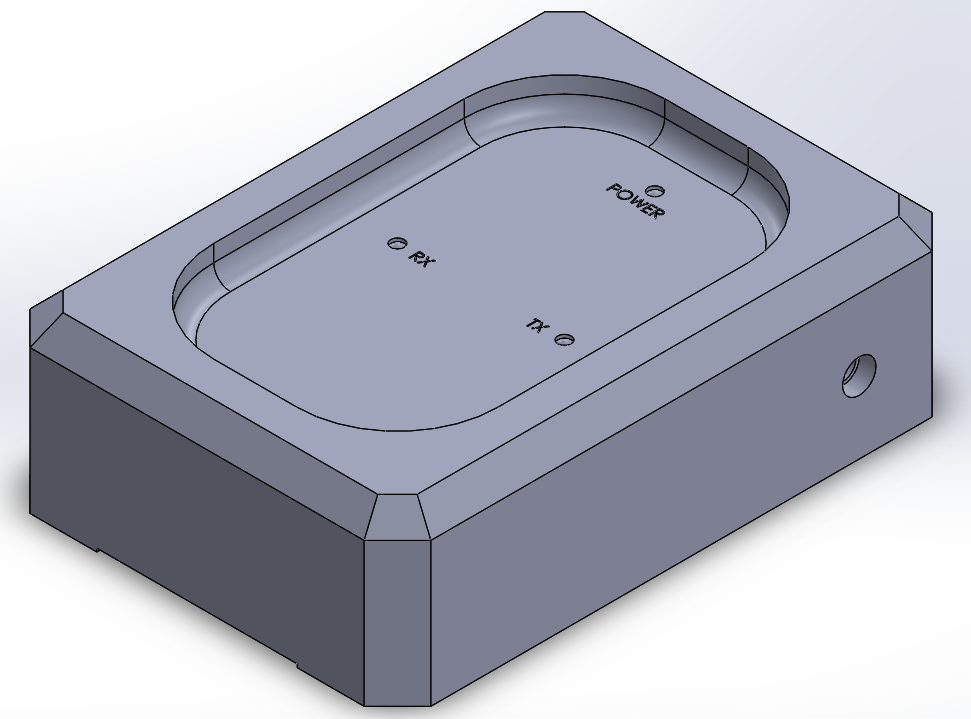
\includegraphics[scale=0.40]{./images/Beacon.png}
    \caption{CAD representation of Beacon}
    \label{Bcn_CAD}
\end{figure}



\pagebreak
\subsection{ID Tag Design}
The ID Tags, the part of the system being tracked by the Beacons, will be powered by a rechargeable 4.5 V battery, which will be charged over time by a RF harvester (see sec. 5.2). The ID Tag will consist of an ESP32 MCU module, and a DWM1000 UWB transceiver chip. The ESP32 is used in the ID tag as it has a function called deep sleep mode, in which the ID Tag has minimum power consumption and does not transmit data for  location tracking. The ID Tag will be activated in an emergency situation via capacitive touch button on the unit. If the button is pressed, and the system is not in an emergency state, the ID Tag will show the charge level and return to deep sleep. However if there is an emergency the ID Tag will then transmit a ping back to the beacon to produce location data as described in the system flow diagram in figure \ref{id_flow}. 

\medskip
\begin{figure}[H]
\centering
    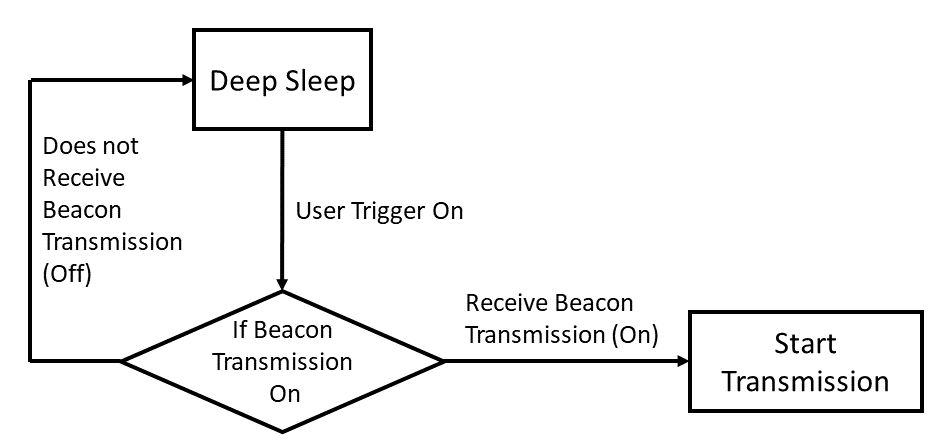
\includegraphics[scale=0.50]{./images/id_flow.png}
    \caption{ID Tag System Flow Diagram}
    \label{id_flow}
\end{figure}
\medskip

A 3D appearance mock-ups of the ID Tag was done in Solidworks and can be seen in the CAD representation, figure \ref{ID_Tag}. The internal components of the ID Tag will be contained in a PLA plastic shell with LEDs indicating the power state, transmission activity, and charge level of the ID Tag. 

\medskip
\begin{figure}[H]
\centering
    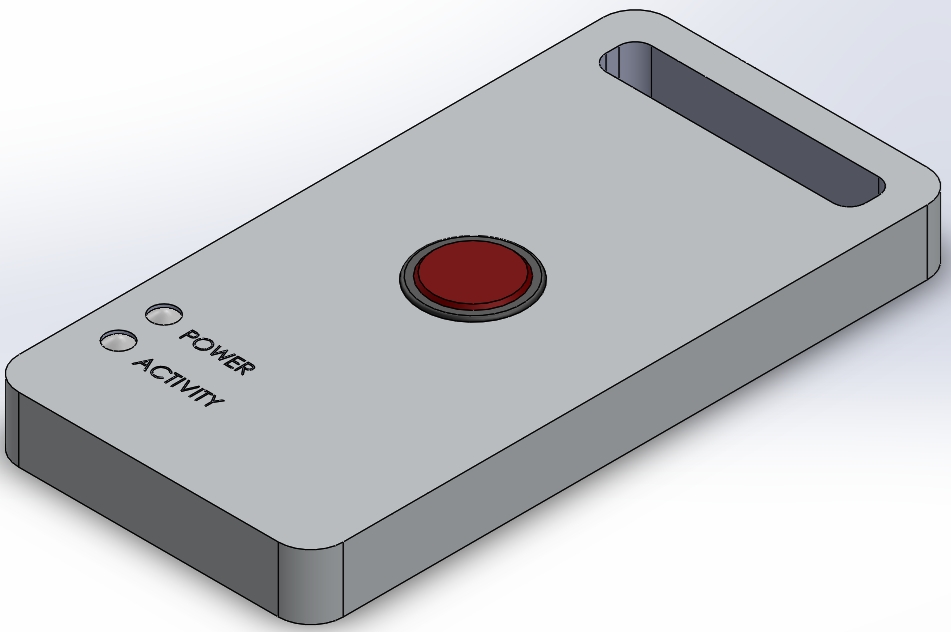
\includegraphics[scale=0.40]{./images/ID_Tag.png}
    \caption{CAD representation of ID Tag}
    \label{ID_Tag}
\end{figure}



\pagebreak
\subsection{Hardware Design Specification}
\medskip
TRIWAVE SYSTEMS has chosen to develop the proof-of-concept prototype using 2.4 GHz Bluetooth radio modules as feasibility testing, before upgrading the system to using Decawave DWM1000 Ultra-Wideband (UWB) modules for further prototyping. ESP32 Micro-controller Units (MCUs) will be used to control the beacons and ID tags and a Raspberry Pi 3 B+ will be used as a data processing unit. The requirements below detail the requirement for hardware functionality of the Akrivia Beacon system.
\medskip
\bgroup
\def\arraystretch{1.5}
\begin{table}[H]
\centering
\begin{tabular}{ | m{3cm} | m{12.5cm} |}
\hline
\textbf{REQ.HW.1 - C} & The Beacons must use ESP32 as the microcontroller unit and transceiver \\
\hline
\textbf{REQ.HW.2 - C} & The ID Tag must use ESP32 as the microcontroller unit and transceiver \\
\hline
\textbf{REQ.HW.3 - P} & ID tag broadcast duration must be at least 1 hour long upon activation\\
\hline
\textbf{REQ.HW.4 - P} & ID tag must return to deep sleep mode after broadcasting period\\
\hline
\textbf{REQ.HW.5 - P} & The Beacons must use Decawave DWM1000 UWB modules as transceivers\\
\hline
\textbf{REQ.HW.6 - P} & The Beacons must use ESP32 as the controller units\\
\hline
\textbf{REQ.HW.7 - P} & The ID tags must use Decawave DWM1000 UWB modules as transceivers\\
\hline
\textbf{REQ.HW.8 - P} & The ID tags must use ESP32 as the controller units\\
\hline
\end{tabular}
\caption{Hardware Design Specification}
\end{table}







